%%%%%%%%%%%%%%%%%%%%%%%%%%%%%%%%%%%%%%%%%%%%%%%%%%%%%%%%%%%%%%%%%%%%%%%%
%                                                                      %
%     File: Thesis_Implementation.tex                                  %
%     Tex Master: Thesis.tex                                           %

%%%%%%%%%%%%%%%%%%%%%%%%%%%%%%%%%%%%%%%%%%%%%%%%%%%%%%%%%%%%%%%%%%%%%%%%

\chapter{Implementation}
\label{chapter:implementation}

\section{Overview}
\label{section:overview}

In this section we describe the implementation of the Binary Level Serialization, Central Serializer, Receiver,
 Message Transportation and Deployment.

%%%%%%%%%%%%%%%%%%%%%%%%%%%%%%%%%%%%%%%%%%%%%%%%%%%%%%%%%%%%%%%%%%%%%%%%
\section{Binary Level Serialization}
\label{section:binaryLevelSerialization}
When we try to work with different computer language and their object types we had problem with serialization.
We can not use standard Java or .Net(C\#) object serialization, because different program languages uses different algoritms
for serialization that's why we’ll run into the problem. for example in our case Java and .Net does'nt use same serialization
algoritm if you serialize an object in Java to binary format and then if you try to deserialize it in .Net language you
will have problem because .Net will not recognize that binary format while deserializing.For example
Person object binary representation is not the same in .Net(Table \ref{tab:netserilazitaon}) and
Java(Table \ref{tab:javaserilazitaon})

\begin{lstlisting}[language=Java, caption={Person Object}]

  public class Person{
       public String name;
       public int age;
  }

\end{lstlisting}

\begin{table}[]
\centering
\begin{tabular}{lllllllllllllll}
0 & 1 & 0 & 0 & 0 & 255 & 255 & 255 & 255 & 1 & 0 & 0 & 0 & 0 & 0 \\
0 & 0 & 12 & 2 & 0 & 0 & 0 & 73 & 83 & 101 & 114 & 105 & 97 & 108 & 105  \\
122 & 97 & 116 & 105 & 111 & 110 & 32 & 116 & 101 & 115 & 116 & 44 & 32 & 86 & 101\\
114 & 115 & 105 & 111 & 110 & 61 & 49 & 46 & 48 & 46 & 48 & 46 & 48 & 44 & 32 \\
67 & 117 & 108 & 116 & 117 & 114 & 101 & 61 & 110 & 101 & 117 & 116 & 114 & 97 & 108 \\
44 & 32 & 80 & 117 & 98 & 108 & 105 & 99 & 75 & 101 & 121 & 84 & 111 & 107 & 101 \\
110 & 61 & 110 & 117 & 108 & 108 & 5 & 1 & 0 & 0 & 0 & 25 & 83 & 101 & 114 \\
105 & 97 & 108 & 105 & 122 & 97 & 116 & 105 & 111 & 110 & 95 & 116 & 101 & 115 & 116 \\
46 & 80 & 101 & 114 & 115 & 111 & 110 & 2 & 0 & 0 & 0 & 21 & 60 & 110 & 97 \\
109 & 101 & 62 & 107 & 95 & 95 & 66 & 97 & 99 & 107 & 105 & 110 & 103 & 70 & 105 \\
101 & 108 & 100 & 20 & 60 & 97 & 103 & 101 & 62 & 107 & 95 & 95 & 66 & 97 & 99 \\
107 & 105 & 110 & 103 & 70 & 105 & 101 & 108 & 100 & 1 & 0 & 8 & 2 & 0 & 0 \\
0 & 6 & 3 & 0 & 0 & 0 & 4 & 74 & 111 & 104 & 110 & 32 & 0 & 0 & 0 \\
11& & & & & & & & & & & & & & &
\end{tabular}
\caption[.Net Serialization Person Object]{.Net Serialization Person Object}
\label{tab:netserilazitaon}
\end{table}


\begin{table}[]
\centering
\begin{tabular}{lllllllllllllll}
  -84 & -19 & 0 & 5 & 115 & 114 & 0 & 23 & 106 & 97 & 118 & 97 & 97 & 112 & 112 \\
  108 & 105 & 99 & 97 & 116 & 105 & 111 & 110 & 55 & 46 & 80 & 101 & 114 & 115 & 111 \\
  110 & 79 & -70 & 94 & 85 & -31 & -32 & -110 & 90 & 2 & 0 & 2 & 73 & 0 & 3 \\
  97 & 103 & 101 & 76 & 0 & 4 & 110 & 97 & 109 & 101 & 116 & 0 & 18 & 76 & 106 \\
  97 & 118 & 97 & 47 & 108 & 97 & 110 & 103 & 47 & 83 & 116 & 114 & 105 & 110 & 103 \\
  59 & 120 & 112 & 0 & 0 & 0 & 32 & 116 & 0 & 4 & 74 & 111 & 104 & 110 \\
\end{tabular}
\caption[Java Serialization Person Object]{Java Serialization Person Object}
\label{tab:javaserilazitaon}
\end{table}

In this case we will use our algoritms instead of using stardard serializer for Java or .Net that both languages could
understand and easily serialize or deserialize.\\

The binary format is always the result of serializing data in each language, with a tag, the number of bytes that follow and
the serialized content. Recovering the serialized data is simply testing the tag to find the data type and then using the
number of bytes and the serialized content. So instead of using stardard serializer with this algoritm we could serialize object
in a language and deserialize with another language.\\

Objects with variables should be serialized to a compound data (composed of inner data). This means having a compound data type,
 with its own tag, and inner components serialized according to their own data type (composition can be recursive).
 This is always recoverable at the receiver, thanks to the tag.\\

In following section CentralSerializer class will help us to seriliaze objects to binary level using primitive type
object serialization.\\


%%%%%%%%%%%%%%%%%%%%%%%%%%%%%%%%%%%%%%%%%%%%%%%%%%%%%%%%%%%%%%%%%%%%%%%%
\section{Central Serializer}
\label{section:centralSerializer}

A message to be sent should be an object (in Java or .Net) that should provide a serialization method, which basically
builds a serialized message (an array of bytes) by sucessively adding each of its components, serialized. This is done by
invoking the methods of the serialization class for primitive data (ints, bools, etc), or by recursively invoking the
serialization method of structured objects that constitute the message.\\

The idea of centralizing the “object of primitive type to a sequence of bytes” and vice-versa methods in a single class
is to avoid the need for every class to have these methods. Since they are static (they receive an object and return bytes,
or vice versa), they can simply be concentrated in a static class (no instances) and invoked from anywhere.\\

The methods to serialize can receive a primitive object (integer, Boolean, etc) and an array of bytes, returning the array
of bytes with the serialized object’s bytes appended. Therefore, each serialization method grows the byte array. When the
user wants to send a message, that message needs to be an instance of a class that has a method that knows how to serialize it,
by invoking the serialization methods of the static class for each of its variables. This needs to be programmed by the use and
is similar to the programming language’s serialization methods.\\

We will show some examples of primitive type serialization.

\begin{figure}[!htb]
  \centering
  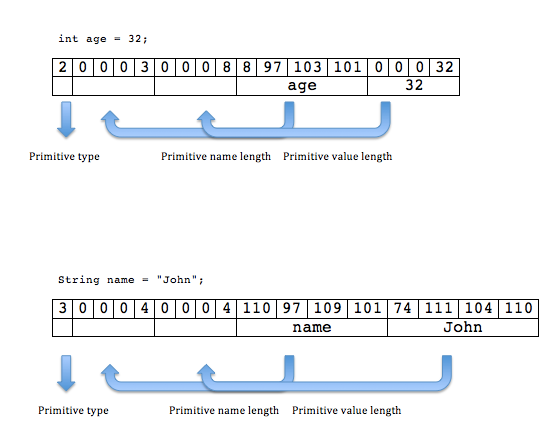
\includegraphics[width=0.9\textwidth]{Figures/binary.png}
  \caption[Examples of primitive type serialization.]{Examples of primitive type serialization.}
  \label{fig:examplebinary}
\end{figure}



%%%%%%%%%%%%%%%%%%%%%%%%%%%%%%%%%%%%%%%%%%%%%%%%%%%%%%%%%%%%%%%%%%%%%%%%
\section{Message Transportation}
\label{section:messageTransfer}

Transferring the array of bytes from sender to receiver requires a binary channel like Web Sockets(HTTP2) or
more classical way by encoding and decoding the binary array with BASE64 and then use typical HTTP-based
solutions (Web Services or REST). The classical solution is of course non-optimal compared to the other ones,
but it can easier to implement given existent tools.\\

Message Transportation in this solution is done with essentially JavaScript and WebSockets [14], to circumvent some of the limitations of HTTP.
The most important issue is that finally humans are also becoming direct Web producers and not merely clients of servers.\\

Web Sockets [44] are fundamental in the efficient support for binary data removes this restriction, increases performance.
They use the protocol upgrade feature of HTTP and
provide a substantial degree of compatibility with existing systems. Part of the HTML5 world, servers and firewalls are
increasingly supporting them and removes this restriction, adds binary support and increases performance.

\begin{figure}[!htb]
  \centering
  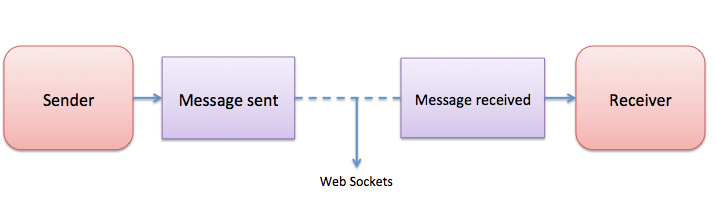
\includegraphics[width=0.5\textwidth]{Figures/websocket.png}
  \caption[Message Transportation.]{Message Transportation.}
  \label{fig:websocket}
\end{figure}
%%%%%%%%%%%%%%%%%%%%%%%%%%%%%%%%%%%%%%%%%%%%%%%%%%%%%%%%%%%%%%%%%%%%%%%%

\section{Receiver}
\label{section:receiver}

The Receving platform makes compliance tests in binary because binary format to be able to traverse both the received message
and each operation’s formal argument, previously serialized. Only the components that match are assigned to the formal argument of the operation.

Two partners will be able to communicate as long as the sender complies with receiver and the receiver conforms to what the
sender expects and it supports all the features that the sender requires, again just in the features actually invoked by the
sender

When the receiver finds a suitable operation, it builds another array of bytes from both the message and the formal argument
then receiver matches components in the formal argument, if it matches it uses the message ones but if not matched by any in the message,
use the ones already in the formal argument

The receiver has always a default value for the message, and only the message components that comply with what the receiver
expects are assigned to the matching receiver argumentís components. Matching in your case is done by name. This means that
the argument (just one) is either primitive (int, bool, string) or structured, with named components. Matching is either the
same type (primitive types) or name by name (if the argument is a structured type).

Then, the platform invokes the operation after generating the argument’s object from array of bytes.
This can be done either by reflection or by invoking a constructor defined by the user in the class of the formal argument,
which knows how to build itself from an array of bytes that respects its components (the new array of bytes respects this
because it was created by copying the original array of bytes of the serialized formal arguments, replacing only the components
 that matched).



%%%%%%%%%%%%%%%%%%%%%%%%%%%%%%%%%%%%%%%%%%%%%%%%%%%%%%%%%%%%%%%%%%%%%%%%

\section{Compliance}
\label{section:compliance}

Compliance is done at the binary level, with primitive components, as we described in previous section. Only the components
that match are assigned to the formal argument of the operation.\\

We should also serialize the formal argument of each operation to make compliance possible. These should also support
optional components which use the formal argument component if none in the message matches it. Therefore, the serialization
methods in the static serialization class should include the name of the component, whether it is optional (a boolean), the type
(encoded in the tag) and the value. For each (primitive) data type can have mandatory annotation.
Messages sent use only mandatory values. Serialized formal arguments can use both mandatory and non-mandatory.

To clarify the compliance, the idea is to serialize the argument (only one, but it can be structured) of each operation of a service
(receiving object). This acts like a default value, against which the message received is matched. A service receiving a message matches
it against the argument of each operation, until it finds one, assigns the message to that argument (partial assignment, see below) and
runs the operation, returning eventually a result.


When checking for compliance, a component in the message with the same name as a component in the operation’s argument matches it and
can be assigned to it (if the message complies with the argument, as a whole). If not, it is ignored. If a component in the argument
is not matched by any of the message’s components and is optional , retains the argument’s value (which acts as a default value).
If all non-optional  components in the argument are matched, there is compliance, the matching components of the message are
assigned to those of the argument with the same name and those that do not match are ignored. Thus the designation partial assignment.

%%%%%%%%%%%%%%%%%%%%%%%%%%%%%%%%%%%%%%%%%%%%%%%%%%%%%%%%%%%%%%%%%%%%%%%%

\section{Deployment}
\label{section:deployment}

The solution is developed and in two different language. They are .NET and Java and deployed Microsoft Azure Cloud. That's way we can
have 2 different provider and .Net client can send message to Java provider over the cloud by using WebSockets and also Java client can
send message to .Net provider. Using Microsoft Azure Cloud allowed us to test project in cloud enviroment
